\section{FF de órbita para perturbação em 60 Hz}

% 2024-07-16-SI_60hz_ff_orbit

\begin{frame}{FF de órbita para perturbação em 60 Hz}

{\footnotesize
\begin{itemize}
    \setlength\itemsep{0.5em}
    \item estudos em 2024-05-14 e 2024-07-01 \href{https://ais-eng-srv-ta.cnpem.br/Olog/index.html\#22801\_4}{\beamergotobutton{Olog \#22801\_4}}
    \item no primeiro estudo, apenas caracterização do FF, sem SOFB.
    \item no segundo estudo testamos nova versão do SOFB com as corretoras no modo \ot{RmpWfm} e agindo no \it{WfmOffsetKick}.
\end{itemize}
}
\vspace{-0.2cm}
\centering
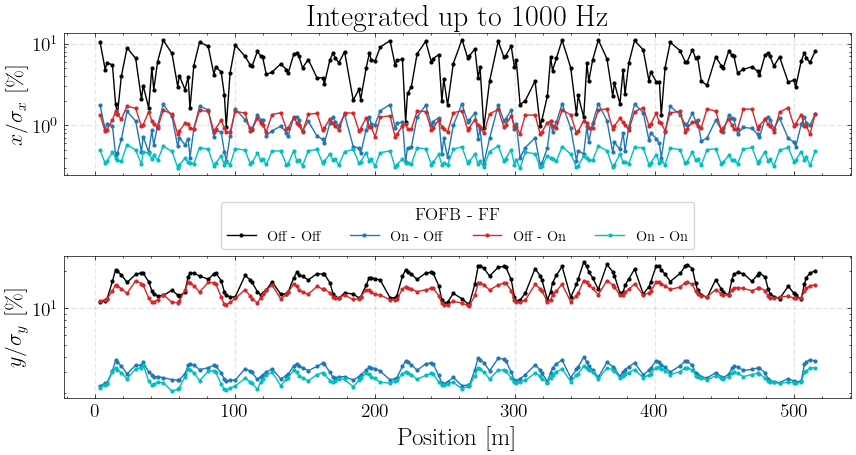
\includegraphics[width=0.7\linewidth]{2024-07-12/figures/integrated_distortion_up_to_1000Hz_run2.png}
\end{frame}
